%************************************************
\chapter{First experiments with Java EE}
\label{ch:first-steps}
%************************************************

\section{Introduction}

The goal of this chapter is to give a first and rapid introduction to the \ac{Java EE} platform. It is to explain how this set of technologies can be used to build and run multi-tiered applications. We introduce concepts, tools and procedures required for building and executing Java EE applications.

\marginpar{The goal of this course is to study design patterns that apply to any multi-tiered application. We use Java EE to illustrate these patterns with concrete implementations, but the concepts are not specific to this technology stack.}

Java EE is only one of the platforms that can be used for building multi-tiered applications. Microsoft .Net is another popular platform based on very similar concepts. There are also related frameworks in Javascript, Python, PHP and other languages.

This chapter introduces a 5-tiers reference architecture and describes the role of every tier at a high level. Every tier will be studied in details in a subsequent chapter. Our goal here is to present the big picture.

In addition to the conceptual overview, we go through concrete operations to get a feel for the developer experience. After reading this chapter, you should have installed at least one of the Java EE application servers, both locally and with Docker. You should also have deployed an existing application, provided to you in the form of an archive file (a \texttt{.war} file). 

\section{Multi-Tiered Applications}

The term \emph{multi-tiered} refers to a particular \emph{style} of \emph{software architecture}. Some applications follow similar patterns in the way they are structured and in the way they interact with external systems. When this is the case, one can say that they follow the same architectural style. In other words, an architectural style is a collection of design constraints and decisions that are common to a class of applications. 

\marginpar{Multi-tiered is a fancy word for describing a distributed application, where a request is issued by a client, received on a server and processed by several components.}

Many applications that are used by professionals and consumers have been designed as multi-tiered applications. Here are some aspects they have in common:

\begin{itemize}
\item An entity uses a device to interact with the application. Think of a user accessing a web application with a browser. Think of a user interacting with a mobile app on his phone. Think of a user typing a command in a Command Line Interface tool. The entity is often a human, but it can also be a script, a robot, a sensor or or an actuator.
\item At some point, the user interaction triggers a call to a \emph{remote} service. This typically happens when the user sends a \emph{query} or a \emph{command} to a remote service. The remote call is made with an application protocol, built on top of a transport protocol. Nowadays, this often means sending a JSON payload over HTTP. But in the early days of Java EE, this often meant making remote method calls from rich clients, with the Java Remote Method Invocation (RMI) protocol.
\item The request is processed by a series of components, which collaborate with each other and focus on a particular task. In other chapters, we will examine the server-side Model View Controller pattern. We will also study different ways to interact with database management systems.
\item During the processing of a request, business logic is executed and the state of the application is retrieved and/or updated. In the end, a response is sent back to the client tier, so that feedback can be presented to the user.
\end{itemize}

A multi-tiered application is a \emph{distributed} application. In general, there is a least one \emph{client} machine and one \emph{server} machine, connected with a network. It is also common to use several machines on the \emph{server} side. For instance, there might be a machine that executes the business logic and another machine that stores data. In addition, one can look at the \emph{physical} and \emph{logical} boundaries between tiers. In other words, when looking at two application components that communicate with each other, one should ask if they are located:

\marginpar{Designing the architecture of a system is about making tradeoffs. Always keep in mind that remote calls are extremely expensive and that interprocess call are very expensive, compared to local method calls. Security, scalability, availability can be arguments for a physical separation, but are they relevant in your application?}

\begin{itemize}
\item on different \emph{machines}
\item on the same machine, but in different \emph{processes}
\item in the same process (they can still be cleanly isolated in \emph{source code packages})
\end{itemize}

Deciding how to split an application and how to use physical and logical tiers can be a bit tricky. It also has a significant impact on non-functional requirements (performance, scalability, security, etc.) and as always, there are pros and cons. In the early days, J2EE guidelines could give the false impression that everything had to be separated. For many simple applications, this translated into higher complexity and lower performance, without clear benefits. Over the years, the community became aware of the design choices and of their implications. Applications developed on top of Java EE became simpler. Logical separation was increasingly preferred to physical separation.

\section{The Five-tiers reference architecture}

The term multi-tiered architecture does not specify how many tiers should be used to organize application components. The client-server architecture is a multi-tiered architecture with 2 tiers. The 3-tiers architecture is a simple model, which emphasizes the separation between the user interface, the business logic and the data persistence. Modern distributed application platforms, such as Java EE or Microsoft .Net often use a more detailed model. These platforms consist of many different APIs and the detailed model is useful to understand where they operate and how they relate to each other. In the case of Java EE, these APIs include the Servlet API, \ac{JSP}, \ac{JAX-RS}, \ac{EJB}, \ac{JPA}, \ac{JMS}, etc.

A graphical representation of the 5-tiers reference architecture is shown in \ref{fig:five-tiers}. The boundaries between the boxes suggest that, very often:

\begin{itemize}
\item the client tier is \emph{far} from the other tiers (they are connected by the Internet)
\item the presentation, business and integration tiers are close to each other (they are often located within the same process)
\item the presentation, business, integration and resources tiers are often connected by the same internal network (calls from the integration to the resources tier are remote, thus quite expensive, but much less expensive than calls that go over the Internet).
\end{itemize}

\begin{figure}[]
	\centering
    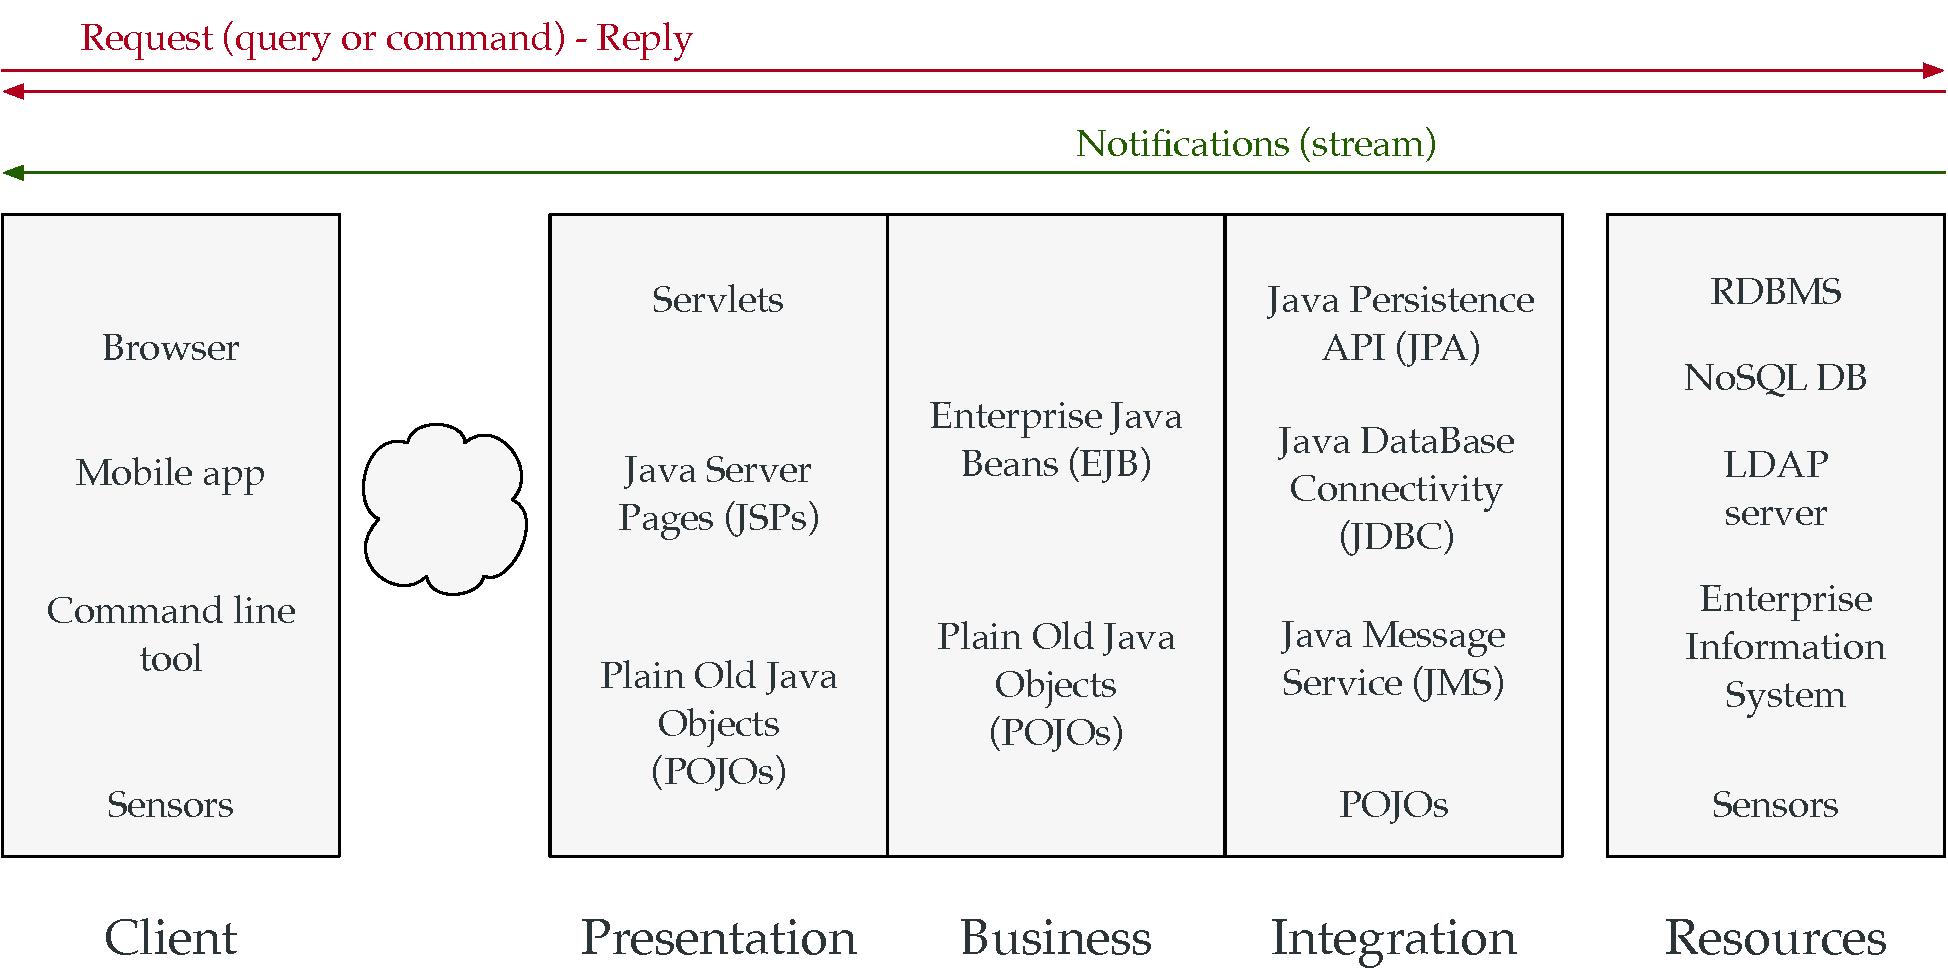
\includegraphics[width=1.0\linewidth]{Figures/tiers.pdf}
	\caption{The five-tiers reference architecture}
  \label{fig:five-tiers}
\end{figure}

\subsection{Client tier}

\marginpar{The client tier represents what I have in my hands.}

The client tier consists of the components that are very close to the user. Typically, the user has some sort of device, such as laptop, a mobile phone or a wearable device. This device provides a runtime environment for our application components. Sometimes, it is the operating system (if we write a standalone client application). Very often, it is a higher-level environment, such as a web browser (which renders our markup pages and runs our client-side Javascript functions).

\subsection{Presentation tier}

\marginpar{The presentation tier is on the server side. It is responsible for accepting requests and generating views.}

The presentation tier is located on the server side, where it provides an entry point. Components in this tier have the responsibility to process incoming requests (e.g. HTTP requests), to delegate work to the business tier and obtain data, and finally to render this data in views that are sent back to the client tier. A common scenario is for the client tier to generate HTML pages, which are then rendered by a browser on the client side. In this case, the page navigation and user interface is managed on the server side. Another common scenario is is for the client tier to generate JSON documents, which are then processed by Javascript components within a browser. In this case, the page navigation and user interface is at least partly managed on the client side. The Single Page Application (SPA) architecture is an example for this scenario.

\subsection{Business tier}

\marginpar{The business tier knows nothing about the user interface, nothing about the protocol used to send client requests. It is purely about business logic.}

The business tier is decoupled from the user interface and is concerned only with business logic. The same business service can serve requests coming from multiple user interaction channels. For instance, in an online shop application, a \emph{shopping cart} service can be used to serve mobile and desktop users.

\subsection{Integration tier}

\marginpar{The integration tier bridges the gap between business logic and data stores.}

The integration tier contains components that make the bridge between business logic and data stores. The integration tier provides an abstraction layer, which means that business services do not interact directly with the data stores. Object-Relational Mapping (ORM) middleware is one way to achieve this goal. In enterprise applications, business services do not only interact with databases. They also interact with other applications, either via connectors or via messaging services. The APIs that support these interactions also fit in the integration tier.

\subsection{Resource tier}

\marginpar{The resource tier is about data stores, but also about external, often legacy, entreprise applications}

The resource tier contains both data stores (databases, directory servers) and external systems that are part of the enterprise information system (e.g. legacy applications). These are the \emph{assets} that the application can use. Are there application components in this tier? It depends on the definition and on the design choices. If all the logic is located in the business tier, then the answer is no. If some of the logic is placed in the data store (e.g. stored procedures in a relational database), then it is yes.

\section{Application servers}

What does it mean for a developer to create a multi-tiered application? How does one create application components that will live in the different tiers? What does it look like in the code, and how does one make this code executable? To answer these questions, it is necessary to understand the role the the application server, which provides a Java EE \emph{runtime} environment.

\marginpar{To execute Java EE code, we need an application server. When we launch it, it accepts HTTP requests on 2 ports. The first port is used for its admin interface. The other port is used for deployed applications. Applications are deployed in the server. When a request arrives, the server forwards the request to one of the deployed applications.}

Before explaining what this means, let us consider what happens with a pure client application built with the Java Standard Edition. Think about a desktop application with a Graphical User Interface or a Command Line Interface. In this case, the code runs directly in the Java Virtual Machine. The user receives a \texttt{.jar} file, containing compiled classes and resources, and types a command such as \texttt{java -jar application.jar} to execute the code. When the command is executed, the JVM starts, loads the classes and executes the \texttt{main} method. The combination of the JVM and of the Java standard library provides a runtime environment: a place where application code can be executed.

With Java EE, the situation is a bit different because the runtime environment offers more APIs and more services. It offers the ability to accept HTTP requests, to interact with databases, to manage security, etc. The runtime environment is provided by an \emph{application server}: a software that implements the Java EE specification (and more) and where applications can be deployed.

As shown in Figure \ref{fig:app-server}, the same server can be used to run multiple applications. It accepts requests on a single TCP port and uses the first element in the path to forward the incoming request to the relevant application. Application servers often provide a web-based administration UI, accessible via a different TCP port. This interface is used to deploy applications, to configure connections to databases and to configure all sorts of technical parameters.

\begin{figure}[]
	\centering
    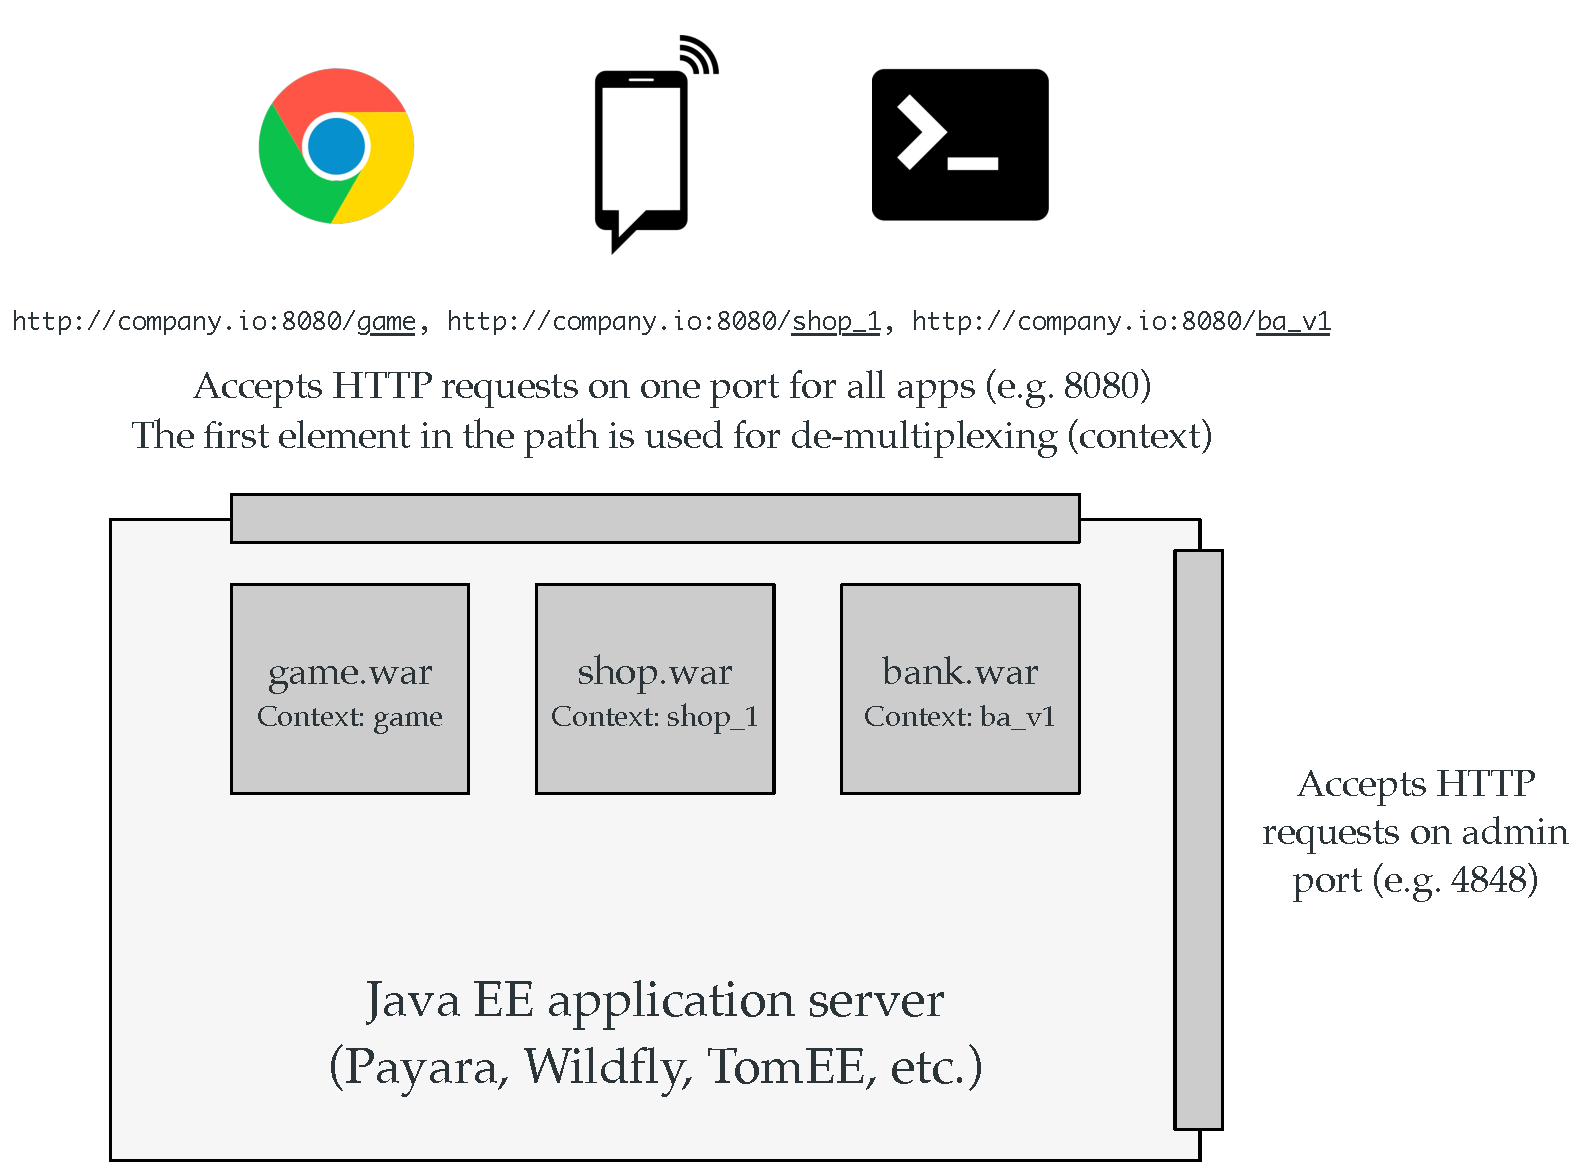
\includegraphics[width=1.0\linewidth]{Figures/app-server.pdf}
	\caption{Applications deployed in a Java EE server}
  \label{fig:app-server}
\end{figure}

\subsection{Java EE, the Java Community Process and Java Specification Requests}

\marginpar{There is not only one company driving the specification of Java EE. There is not only one company providing the implementation of the specification.}

Java Enterprise Edition was designed as a standard platform, through the \emph{Java Community Process}. This means that expert groups, with representatives from different companies, have first written the specifications for the different aspects of the platform. The term \emph{Java Specification Request} (JSR) refers to one such specification: there are JSRs related to presentation-tier technologies (e.g. Servlet, JSP, JAX-RS), there are JSRs related to business-tier concerns (e.g. EJB), etc. Note that the JCP is not only used for Java EE APIs, but for the Java platform in general.

\marginpar{A JSR is similar to an RFC: it is the specification of an open standard. Companies and open source communities can then build compatible (and competing) implementations.}

The standardization process means that when a JSR has been defined, different companies and open source communities can provide a competing implementation of the specification. This means that when you decide to use a particular JSR, you also need to decide which implementation you want to use.
 
\subsection{Choosing an application server}

In the early 2000s, most application servers were commercial servers sold by companies like IBM, BEA and Sun Microsystems. They were expensive and were targeting enterprise customers. In the mid 2000s, open source implementations became viable alternatives. Today, many enterprise customers have moved away from commercial implementations and use open source servers.

The following list is not exhaustive, but gives an overview of available servers:

\begin{itemize}
\item \emph{Wildfly}: an open source application server developed by Red Hat. Open source, free, leading edge.
\item \emph{JBoss Enterprise Application Platform}, also provided by Red Hat. Commercial support, certified.
\item \emph{Glassfish}: initially developed by Sun Microsystems, former reference implementation. Used to work very well, but was killed by Oracle.
\item \emph{Payara}: fork of the Glassfish codebase, developed by the Payara Foundation. Addresses issues with last versions of Glassfish, aims to become a leader in the future Java EE versions.
\item \emph{Apache Tomcat}: strictly speaking, not a Java EE application server because it only implements a subset of the Java EE APIs. Extremely popular and very often used to deploy applications built with the Spring Framework.
\item \emph{Apache TomEE}: the combination of Tomcat and OpenEJB, OpenJPA, MyFaces to fill the gap between Tomcat and the full Java EE specification.
\item \emph{WebLogic}: previously developed by BEA, then acquired by Oracle. Used to be an expensive and popular solution. 
\item \emph{Websphere}: developed by IBM. Price wise, in the same category as WebLogic.
\end{itemize}

\marginpar{Suggestion: experiment with Wildfly, Payara and TomEE. Make sure that you understand how to deploy a .war file in each of the Java EE application servers. Pick your favorite and dig deeper in the configuration.}

To get familiar with Java EE development, it is worth experimenting with 2 or 3 different application servers. This helps understand what is defined in the specification and common to all application servers. This also helps realize that some aspects are not defined in the specifications (e.g. what configuration interface should be provided), and that every application server is free to provide additional features.

As of today, we recommend to experiment with Payara, Wildfly and Tomcat/TomEE. Depending on your preferences, we then recommend that pick one of them and dig into the details of the administration and configuration interfaces.

\subsection{Installing and running an application server}

There are two ways to get one of these application servers up and running:

\marginpar{A demonstration of the installation process is available in the Webcast. Be aware that it was recorded with previous versions of the application servers.}

\begin{itemize}
\item Today, there is an official Docker image for every open source server. The documentation of the images give instructions for running a container and performing basic configuration (in many cases, it is necessary to create user accounts to get access to the administration console). The great thing about this method is that you can get started within minutes. The other great thing is that you have a way to package and distribute your applications, by creating your own Docker images.
\item For developers, it is sometimes better to have a local installation of the application server. This enables some features in the IDE and makes the development cycle more efficient. The three open source application servers are very easy to install: the process essentially consists of extracting an archive file and running a script in a bin directory.
\end{itemize}


\section{The Java EE development cycle}

\marginpar{Having silos in the organization and a clear separation between development and IT operations used to be the norm. This has proven to cause many problems. The trend is to break these barriers and to work in small autonomous teams. This is a core principle in the DevOps approach.}

The original Java 2 Enterprise Edition specification described a complete software development lifecycle, with clearly defined engineering roles. In the early days, it made the boundaries between \emph{building} software and \emph{running} software very explicit. This reflected the organization of most companies at the time, who had separate \emph{development} and \emph{IT operations} teams. In this model:

\begin{itemize}
\item software engineers were responsible for building components and applications. Ideally, they should be able to focus on business logic and not worry (too much) about technical challenges. In theory, they should be able to \emph{declare} the non-functional requirements of their applications (availability, security, etc) and let the runtime environment take care of the rest.
\item IT ops engineers were responsible for running these applications. They were responsible for designing (often distributed) runtime environments, for deploying applications and for making sure that they kept working. IT ops were the engineers carrying pagers and dealing with production issues.
\end{itemize}

\marginpar{A .war file is almost the same thing as a .jar file. It is an archive, which contains compiled classes, resources and metadata. The structure of folders and the name of files is defined in the specification.}

In this model, how do software and IT ops engineers collaborate? What happens when a new feature has been developed, or when a bug has been fixed in the source code? Depending on the environment and the type of application, this can be a complex process. One aspect of this process is to have a way to \emph{package} enterprise application in some sort of archive, which can be produced by software engineers and delivered to IT ops engineers. 

When Java EE was created, the Java platform had already defined a format for creating packages: the \emph{Java ARchive} format. Java developers are familiar with \emph{.jar} files, which contain compressed .class files, resources and metadata information. These files are used to distribute libraries and applications executed directly in the Java Virtual Machine. The same approach was used for Java EE and several related archive formats have been proposed:

\begin{itemize}
\item The \emph{WAR} format was proposed for web applications. In the early days, the intent was to package \emph{presentation-tier} components in these archives. In other words, the components that process HTTP requests, obtain some data and generate views that are sent in HTTP responses. As we will see later, this meant Servlets, Java Server Pages (JSPs) and helper Plain Old Java Object (POJO) classes. 
\item The \emph{JAR} format was proposed for business components. The idea was to design components that would be decoupled from the presentation tier and could be reused across different user interface channels. These components would need to interact with databases, legacy applications and messaging platforms. They would often require a way to deal with distributed transactions. We we will see, Enterprise Java Beans (EJBs) have been developed for this purpose. EJBs are packaged in .jar files.
\item The \emph{EAR} format was proposed for entire applications. For many years, the way to build Java EE applications was to create separate packages for the web tier (in a .war file) and the business tier (in one or more .jar files). All these components were then assembled in a larger .ear file, which contained extra metadata.
\end{itemize}

\marginpar{In the past, developers had to create .ear files, which contained .war and .jar files. The These archives reflected the tiers of the application. Today, it is possible and more common to put all application components in a simpler .war file. Separation between tiers is visible in the source code package structure.}

It is important to be aware of the original \emph{.ear} packaging model for Java EE applications, because there are still many legacy applications that are built on this model. For a Java developer, there is still a high probability to encounter such an application. But it is also important to understand that over the years, the original model has been revised several times, with the goal to provide a more lightweight experience to developers. For many years, most teams have dropped the EAR format and only use the WAR format. Indeed, it is not possible to put Enterprise Java Beans (EJBs) together with the presentation tiers. In addition, many developers have made the choice not to use EJBs and develop business services with POJOs and the help of frameworks such as the Spring Framework.

\section{Online resources}

The following resources are available for this chapter:

\begin{itemize}
\item In the companion \href{https://www.youtube.com/playlist?list=PLfKkysTy70QaWqP7sD6xiqFvLZemVLQw_}{YouTube playlist}, the sequence of four videos entitled \emph{Bootcamp 1.1} to \emph{Bootcamp 1.4} present the Java EE development workflow and demonstrate how to deploy the same .war file in three different application servers. The videos were recorded in 2016, so be aware that the versions of the servers are outdated. Some of the operations might be slightly different. Also, instead of using Glassfish, we recommend that you switch to Payara.
\item On GitHub, the repo \href{https://github.com/SoftEng-HEIGVD/Teaching-HEIGVD-AMT-Discovery}{SoftEng-HEIGVD/Teaching-HEIGVD-AMT-Discovery} contains the \texttt{.war} file used in the webcasts. You need to clone in order to go through the tutorial steps. The repo also contains Docker configuration.
\end{itemize}



\section{Questions}

To answer these questions, you will need to have read the chapter but also to have done some research. Make sure that you are able to answer every question. Discuss your responses with your peers.

\begin{enumerate}
\item \emph{Is Apache Tomcat an application server?} The answer to this question depends on the definition of \emph{application server}. Explain why it is correct to answer positively and negatively to the question.
\item \emph{What is the role of a .war file?} Explain how it fits in the Java EE development model and bridges the gap between development and operations.
\item \emph{Is the J2EE development model an anti-pattern?} On paper, the clear separation between development and operations teams makes sense. However, the current trends in the industry are very different. Explain how modern practices give a different perspective on the question.
\item What is the difference between the \emph{client} tier and the \emph{presentation} tier. They both seem to be related to the user interface, so why are they both needed?
\item Consider the web site \texttt{https://qoqa.ch}. It is reasonable to think that it is built on a multi-tiered architecture. Use the 5-layers diagram and draw the components that might be part of the system. 
\item We have stated that components in the business tier should be decoupled from the user interface. Use the 5-layers diagram and describe a scenario that shows how a business service can be reused across interaction channels.
\item Most application servers provide 3 ways to deploy a \texttt{.war} file. Describe how these methods work and what are there benefits and drawbacks.
\end{enumerate}
